\documentclass[]{beamer}
\usepackage[T1]{fontenc}
\usepackage[utf8]{inputenc}
\usepackage{lmodern}
\usepackage[italian]{babel}
\usepackage{mathrsfs}
\usepackage{cancel}

\title{Momento}
\author{\texorpdfstring{Mattia Cozzi\newline\href{mailto:cozzimattia@gmail.com}{\texttt{cozzimattia@gmail.com}}}{Mattia Cozzi}}
\date{a.s.~2023/2024}

%\documentclass[handout]{beamer}     %usare questa classe per generare l'handout
%\usepackage{pgfpages}   %per mostrare più quadri nella stessa pagina
%\pgfpagesuselayout{4 on 1}[a4paper,border shrink=5mm,landscape]
\usetheme{Singapore}
%\useoutertheme[left]{sidebar} %elementi intorno alle diapositive
\setbeamercovered{dynamic} %modifica l'aspetto del testo grigetto delle diapositive future. Argomenti: invisible/transparent/dynamic
\usecolortheme{orchid}
%COLORE PRINCIPALE
% \definecolor{marroncino}{RGB}{156, 26, 0} % UBC Blue (primary)
% \setbeamercolor{structure}{fg=marroncino} % itemize, enumerate, etc

\theoremstyle{plain}
\newtheorem{teorema}{Teorema}

\usepackage{tikz}
\usepackage{circuitikz}

\usepackage{pgf,pgfplots,graphicx}
\usetikzlibrary{angles,quotes,arrows,shapes,decorations.markings}
\pgfplotsset{compat=1.15}
\usepgfplotslibrary{units,fillbetween} % to add units easily to axis

\newcommand{\fem}{f_{em}}

\def\angolo[#1](#2)(#3:#4:#5)% Syntax: [draw options] (center) (initial angle:final angle:radius)
    { \draw[#1] ($(#2)+({#5*cos(#3)},{#5*sin(#3)})$) arc (#3:#4:#5); }


\newcommand<>{\xxcancel}[1]{\alt#2{\xcancel{#1}\vphantom{#1}}{#1}}

\begin{document}

\begin{frame}
  \titlepage
\end{frame}





\begin{frame}
\frametitle{Contenuti}
\tableofcontents
\end{frame}


\section{Momento di una forza}

\begin{frame}
\frametitle{Rotazioni}
Per descrivere il modo in cui le forze agiscono su corpi estesi (come una penna o una porta) introduciamo un nuovo concetto, considerando anche il \alert<1>{punto di applicazione} della forza.\pause

~

Utilizzeremo:
\begin{itemize}
  \item la \alert<2>{forza $ \vec{F} $}, applicata in un certo punto dell'oggetto;\pause
  \item il \alert<3>{punto $ O $}, scelto a piacimento (spesso è il centro della rotazione dell'oggetto);\pause
  \item il \alert<4>{vettore $ \vec{r} $} (braccio della forza), che collega $ O $ al punto di applicazione della forza.
\end{itemize}
\begin{figure}
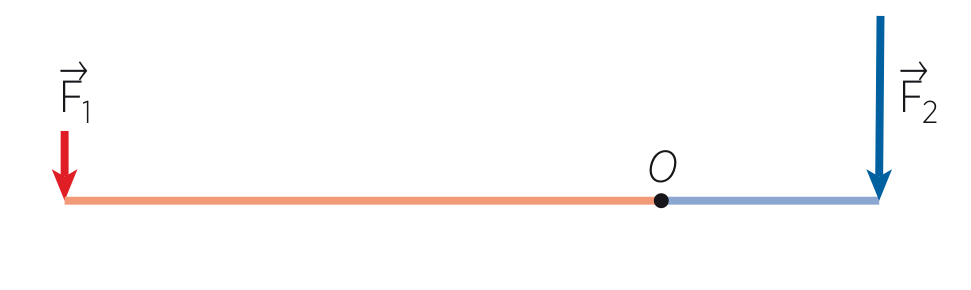
\includegraphics[width=.5\columnwidth]{img/braccioforza.png}
\end{figure}
\end{frame}


\begin{frame}
\frametitle{Momento di una forza (momento torcente)}
\begin{block}{Momento di una forza}
Il momento (torcente) $ \vec{M} $ della forza $ \vec{F} $ rispetto al punto $ O $ è il prodotto vettoriale tra il braccio e la forza:
\begin{center}
\colorbox{blue!30}{$ \vec{M} = \vec{r} \times \vec{F} $}
\end{center}\pause
Il modulo del momento si calcola con:
\begin{center}
$ M = rF\sin\theta $
\end{center}
dove $ \theta $ è l'angolo tra $ \vec{r} $ e $ \vec{F} $.
\end{block}
\end{frame}



\begin{frame}
\frametitle{Il ruolo dell'angolo}

\begin{columns}
\begin{column}{0.3\textwidth}
\begin{figure}
\begin{tikzpicture}[scale=.5,rotate=0]
\angolo[black](1.5,-.5)(0:90:.8)
\node [left,thick] at (2.2,.6) {{\tiny $ \theta $}};
\node [left,blue,thick] at (1.5,1) {{\tiny $ \vec{F} $}};
\draw [->,blue,thick] (1.5,-.5) -- (1.5,2);
\node [left,red,thick] at (3.5,0) {{\tiny $ \vec{r} $}};
\draw [<-,red,thick] (1.5,-.5) -- (3,-.5);
\end{tikzpicture}

~

{\footnotesize $ \sin\theta = 1 $\\momento massimo

~

forza efficace}
\end{figure}
\end{column}
\begin{column}{0.3\textwidth}
\vspace{.82cm}
\begin{figure}
\begin{tikzpicture}[scale=.5,rotate=270]
\angolo[black](1.5,-.5)(270:90:.8)
\node [above,thick] at (.8,-.5) {{\tiny $ \theta $}};
\node [above,blue,thick] at (1.5,1.5) {{\tiny $ \vec{F} $}};
\draw [->,blue,thick] (1.5,-.5) -- (1.5,2.5);
\node [below,red,thick] at (1.5,-1.5) {{\tiny $ \vec{r} $}};
\draw [<-,red,thick] (1.5,-.5) -- (1.5,-2.5);
\end{tikzpicture}

{\footnotesize $ \sin\theta = 0 $\\momento nullo

~

forza inefficace}
\end{figure}



\end{column}
\begin{column}{0.3\textwidth}
\vspace{1.29cm}
\begin{figure}
\begin{tikzpicture}[scale=.5,rotate=307]
\angolo[black](1.5,-.5)(52:90:.8)
\node [above left,thick] at (2.3,.6) {{\tiny $ \theta $}};
\node [left,blue,thick] at (1.4,1.2) {{\tiny $ \vec{F} $}};
\draw [->,blue,thick] (1.5,-.5) -- (1.5,2);
\node [above,red,thick] at (3.5,.8) {{\tiny $ \vec{r} $}};
\draw [<-,red,thick] (1.5,-.5) -- (3,1.5);
\end{tikzpicture}

{\footnotesize $ 0 < \sin\theta < 1 $\\momento ``intermedio''

~

forza parzialmente efficace}
\end{figure}
\end{column}
\end{columns}
\end{frame}



\begin{frame}
\frametitle{Esercizio}
\begin{exampleblock}{Pedalata}
  \small{Al pedale di una bicicletta è applicata una forza di $ 100 \, N $ con un angolo di inclinazione di $ 60^\circ $, che produce un momento di $ 8,5 \, N/m $.

  A quale distanza dal centro di rotazione è applicata la forza?\hspace*{\fill}[$ 10 \, cm $]}
\end{exampleblock}
\end{frame}




\begin{frame}
\frametitle{Il vettore momento torcente}
Essendo $  \vec{M} =\vec{r}\times\vec{F} $ un vettore, dobbiamo ancora indicarne:\pause
\begin{columns}
\begin{column}{0.5\textwidth}
\begin{itemize}
\item \alert{direzione}, \emph{normale} al piano determinato da $ \vec{r} $ e da $ \vec{F} $;\pause
\item \alert{verso}, dato dalla \emph{regola della mano destra}.\pause
\end{itemize}

~\\~\\~\\~\\~
\end{column}
\begin{column}{0.5\textwidth}

\begin{figure}
\begin{tikzpicture}[scale=1]
\fill[fill=red!10] (0,0) -- (4,0) -- (3,-1) -- (-1,-1) -- cycle;
\draw [<-,thick,blue] (0,0) -- (4,0);
\node [below,blue] at (1,-1) {$ \vec{F} $};
\node [below right] at (0,0) {$ O $};
\draw [->,thick,red] (0,0) -- (-1,-1);
\node [above left,red] at (-.5,-.5) {$ \vec{r} $};
\draw [->,orange,thick] (0,0) -- (0,3);
\node [right,orange,thick] at (0,2) {$ \vec{M} $};
\draw (.3,0) -- (.3,.3);
\draw (.3,.3) -- (0,.3);
\draw (0,.3) -- (-.2,.1);
\draw (-.2,.1) -- (-.2,-.2);
\draw [ultra thick,fill] (0,0) circle [radius=.015];
\end{tikzpicture}
\end{figure}
\end{column}
\end{columns}
\end{frame}


\begin{frame}
\frametitle{Regola della mano destra}
\begin{figure}
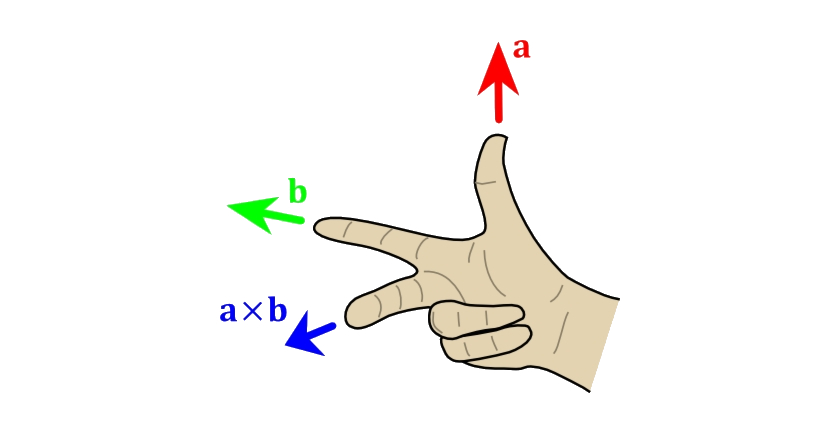
\includegraphics[width=\columnwidth]{img/manodestra.jpg}
\end{figure}
\end{frame}



\begin{frame}
\frametitle{Esempio}
\begin{figure}
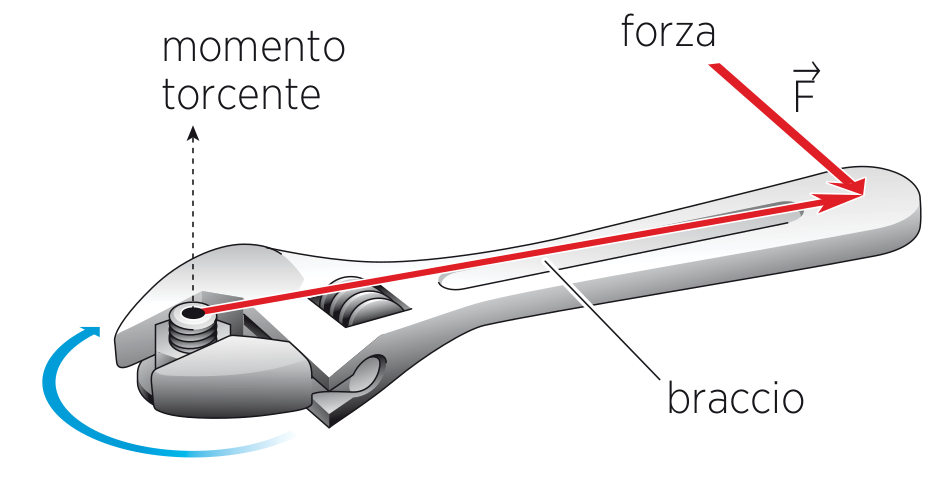
\includegraphics[width=.7\columnwidth]{img/chiaveinglese.png}
\end{figure}
\end{frame}









\section{Momento angolare}


\begin{frame}
\frametitle{Momento angolare (1)}
Per descrivere i moti di rotazione, introduciamo il momento angolare.\pause
\begin{block}{Momento angolare}
Il momento angolare $ \vec{L} $ di una particella rispetto al punto $ O $ è il prodotto vettoriale tra il raggio vettore e la quantità di moto della particella.
\begin{center}
\colorbox{blue!30}{$ \vec{L} = \vec{r} \times \vec{p} $}
\end{center}\pause
Il modulo del momento si calcola con $ L = rp\sin\theta $, dove $ \theta $ è l'angolo tra $ \vec{r} $ e $ \vec{p} $.
\end{block}\pause
Valgono le stesse considerazioni fatte per $ \vec{M} $.
\end{frame}


\begin{frame}
\frametitle{Momento angolare (2)}
\begin{columns}
\begin{column}{0.5\textwidth}
\visible<1->{
\begin{figure}
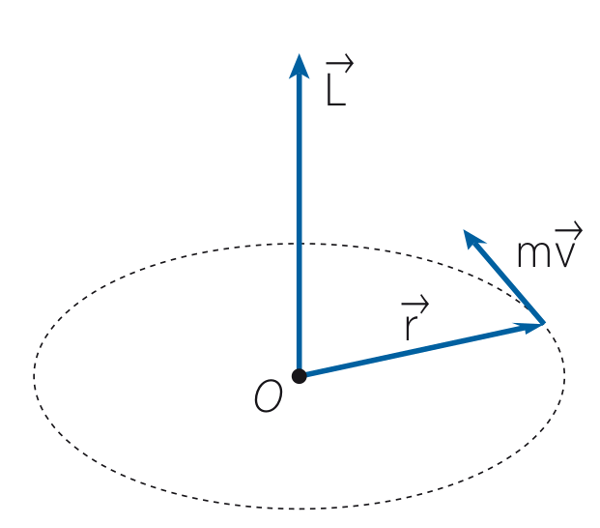
\includegraphics[width=.7\columnwidth]{img/momang1.png}
\end{figure}}
\end{column}
\begin{column}{0.5\textwidth}
\visible<2>{
\begin{figure}
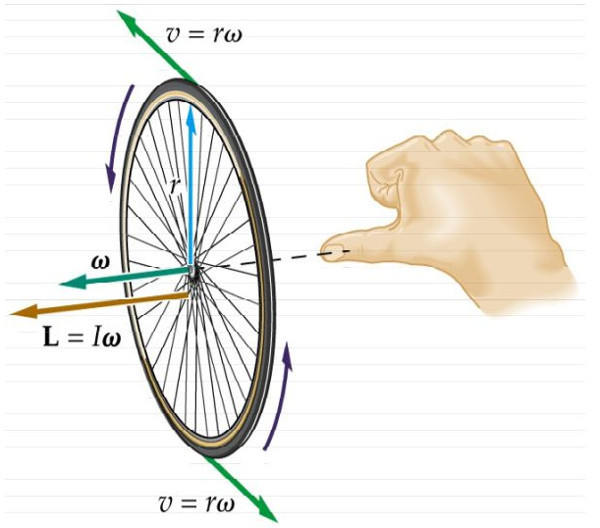
\includegraphics[width=.7\columnwidth]{img/momang2.jpg}
\end{figure}}
\end{column}
\end{columns}
\end{frame}



\section{Conservazione}

\begin{frame}
\frametitle{Conservazione del momento angolare}
Per il momento angolare (così come per la quantità di moto) vale il principio di:
\begin{block}{Conservazione del momento angolare}
Se un sistema è isolato (cioè su di esso non agiscono forze esterne) il momento angolare totale del sistema si conserva.
\end{block}\pause

~

Poiché il momento angolare è un vettore, si conservano anche la sua direzione e il suo verso. Oggetti che ruotano tendono pertanto a rimanere sullo stesso piano.

\begin{center}
\href{video/Conservazionemomento.mp4}{\beamergotobutton{Video: Conservazione del momento angolare}}
\end{center}
\end{frame}

\begin{frame}
\frametitle{Variazione tramite momento torcente}
Sappiamo che se su un corpo agisce una forza $ \vec{F} $ per un tempo $ \Delta t $, allora si ha una variazione della quantità di moto $ \Delta\vec{p} $.
\begin{center}
Teorema dell'impulso

$ \Delta\vec{p} = \vec{F}\Delta t $
\end{center}\pause

~

Per variare il momento angolare di un corpo, è necessario applicare un \alert<2>{momento torcente $ \vec{M} $} per un tempo $ \Delta t $.
\begin{center}
\colorbox{blue!30}{$ \Delta \vec{L} = \vec{M}\Delta t $}
\end{center}
\end{frame}


\begin{frame}
\frametitle{Esercizio}
\begin{exampleblock}{Lancio del martello}
  \small{Un lanciatore di martello scaglia il suo attrezzo dopo averlo fatto accelerare per $ 2,0 \, s $ applicandogli una forza media di $ 35 \, N $ tangente alla traiettoria. Il martello pesa $ 2,5 \, kg $ e la catena a cui è attaccato è lunga $ 90 \, cm $.
  \begin{itemize}
    \item Quanto vale il momento angolare del martello al momento del lancio?\hspace*{\fill}[$ 63 \, kg\cdot m^2 /s $]
    \item A che velocità viene lanciato il martello?\hspace*{\fill}[$ 28 \, m/s $]
  \end{itemize}

  }
\end{exampleblock}
\end{frame}



\begin{frame}
\frametitle{Moti di traslazione e moti di rotazione (1)}
\centering
\begin{tabular}{c|c}
\textbf{Traslazione} & \textbf{Rotazione} \\\rule{0pt}{5ex}
$ \vec{F} $ & $ \vec{M} = \vec{r} \times \vec{F} $ \\\rule{0pt}{5ex}
$ \vec{p} = m\vec{v} $ & $ \vec{L} = \vec{r} \times \vec{p} = \vec{r} \times m\vec{v} $ \\\rule{0pt}{5ex}
$ \Delta \vec{p} = \vec{F}\Delta t $ &  $ \Delta \vec{L} = \vec{M}\Delta t $ \\
  \end{tabular}
\end{frame}

\section{Momento d'inerzia}


\begin{frame}
\frametitle{Momento d'inerzia}
Sappiamo che la \alert<1>{massa inerziale $ m $} quantifica la resistenza di un corpo alla variazione della sua velocità (di traslazione).\pause

~

L'analogo per i moti di rotazione è il \alert{momento d'inerzia $ I $}, che quantifica la resistenza di un corpo al variare la sua velocità angolare $ \omega $.\pause

~

Il momento d'inerzia di un corpo esteso dipende dalla specifica forma del corpo.
\begin{center}
\href{gif/momentoinerzia.gif}{\beamergotobutton{GIF: Momento d'inerzia di diversi corpi}}
\end{center}
\end{frame}


\begin{frame}
\frametitle{Momento angolare e momento d'inerzia}
Il momento d'inerzia è legato al suo momento angolare dalla relazione:
\begin{center}
\colorbox{blue!30}{$ \vec{L} = I \vec{\omega} $}
\end{center}\pause

~

Tale relazione è l'analogo di $ \vec{p} = m\vec{v} $.
\end{frame}

\begin{frame}
\frametitle{Velocità di rotazione}
Notiamo che \alert<1>{il momento d'inerzia è direttamente proporzionale al quadrato delle dimensioni del corpo}.\pause

~

Se durante una rotazione cambiamo le dimensioni del corpo, possiamo variarne la velocità angolare:
\begin{center}
$ L_1 = L_2 $\pause

~

$ I_1 \omega_1 = I_2 \omega_2 $
\end{center}
\alert<3>{Se $ I $ diminuisce, $ \omega $ aumenta} (o viceversa).
\begin{center}
\href{video/Conservazionemomento2.mp4}{\beamergotobutton{Video: Variazione della velocità angolare in un sistema isolato}}
\end{center}
\end{frame}


\begin{frame}
\frametitle{Esercizio}
\begin{exampleblock}{Velocità angolare e momento d'inerzia}
  \small{Una pattinatrice ferma in mezzo alla pista sta facendo una piroetta con le braccia distese e con velocità angolare di intensità $ 3,50 \, rad/s $. Ad un certo punto raccoglie le braccia intorno al corpo, in modo che il suo momento d'inerzia si dimezzi.
  
  Quanto vale ora il modulo della sua velocità angolare?%\hspace*{\fill}[$ 7,00 \, rad/s $]
  }
\end{exampleblock}
\end{frame}

\section{Energia}

\begin{frame}
\frametitle{Energia cinetica rotazionale}
Un corpo in rotazione possiede una certa \alert<1>{energia cinetica rotazionale}:
\begin{center}
\colorbox{blue!30}{$ K = \dfrac{1}{2} I \omega^2 $}
\end{center}\pause

~

Tale relazione è l'analogo di $ K = \dfrac{1}{2} m v^2 $.
\end{frame}





\section{Dinamica rotazionale}

\begin{frame}
\frametitle{Accelerazione angolare e momento}
Se un corpo varia la sua velocità angolare, allora subisce una \alert<1>{accelerazione angolare}:
\begin{center}
\colorbox{blue!30}{$ \vec{\alpha} = \dfrac{\Delta \vec{\omega}}{\Delta t} $}
\end{center}\pause

~

È possibile ora dimostrare che:
\begin{center}
\colorbox{blue!30}{$ \vec{M} = I\vec{\alpha} $}
\end{center}
\end{frame}


\begin{frame}
\frametitle{Dimostrazione }
Rispetto alla variazione del momento angolare, sappiamo che:
\begin{center}
$ \Delta \vec{L} = \vec{M}\Delta t $~~~~~~~~e~~~~~~~~$ \Delta \vec{L} = I \Delta\vec{\omega} $ \pause

~

$ \vec{M}\Delta t = I \Delta\vec{\omega} $\pause

~

$ \vec{M} = I \dfrac{\Delta\vec{\omega}}{\Delta t} $\pause

~

\colorbox{blue!30}{$ \vec{M} = I \vec{\alpha} $}
\end{center}\pause
La relazione dimostrata è l'analogo di $ \vec{F} = m \vec{a} $.
\end{frame}

\begin{frame}
\frametitle{Moti circolari}

\begin{columns}
\begin{column}{0.5\textwidth}
\visible<1->{
\begin{center}
Legge oraria del moto circolare\\a velocità costante

~

\colorbox{blue!30}{$ \theta(t) = \omega t + \omega_0 $}

~

~

Analogo di:

$ s(t) = vt + s_0 $
\end{center}
}
\end{column}
\begin{column}{0.5\textwidth}
\visible<2>{
\begin{center}
Legge oraria del moto circolare\\accelerato

~

\colorbox{blue!30}{$ \theta(t) = \dfrac{1}{2}\alpha t^2 + \omega_0 t + \omega_0 $}

~

~

Analogo di:

$ s(t) = \dfrac{1}{2}at^2 + v_0 t + s_0 $
\end{center}
}
\end{column}
\end{columns}



\end{frame}


\begin{frame}
\frametitle{Moti di traslazione e moti di rotazione (2)}
\centering
\begin{tabular}{c|c}
\textbf{Traslazione} & \textbf{Rotazione} \\\rule{0pt}{4ex}
$ m $ & $ I $ \\\rule{0pt}{3ex}
$ \vec{v} $ & $ \vec{\omega} $ \\\rule{0pt}{3ex}
$ \vec{a} $ & $ \vec{\alpha} $ \\\rule{0pt}{4ex}
$ \vec{F} = m\vec{a} $ & $ \vec{M} = I\vec{\alpha} $ \\\rule{0pt}{4ex}
$ \vec{p} = m\vec{v} $ & $ \vec{L} = I\vec{\omega} $ \\\rule{0pt}{4ex}
$ \Delta \vec{p} = \vec{F}\Delta t $ &  $ \Delta \vec{L} = \vec{M}\Delta t $ \\\rule{0pt}{4ex}
$ K = \frac{1}{2} I \omega^2 $ & $ K = \frac{1}{2} m v^2 $ \\
  \end{tabular}
\end{frame}




\end{document}
